%! TEX root = ../../master.tex
\lecture[Efficient 2-Matroid intersection algorithm. Bipartite matching as an application. 3-Matroid is $\NPC$. Further thoughts on Totally Dual Integrality.]{Tu 24 May 2022}{Matroid intersection}

Further consider
\begin{align*}
    S_1 & \coloneqq \{e \in I^c \mid I + e \in \mathcal I_1\}, \\
    S_2 & \coloneqq \{e \in I^c \mid I + e \in \mathcal I_2\}.
\end{align*}
\begin{example}
    Consider a bipartite matching and its matroid-intersection graph for some
    independent set $I \subseteq \mathcal I_1\cap \mathcal I_2$:
    \\
    \begin{minipage}{\textwidth}
        \centering
        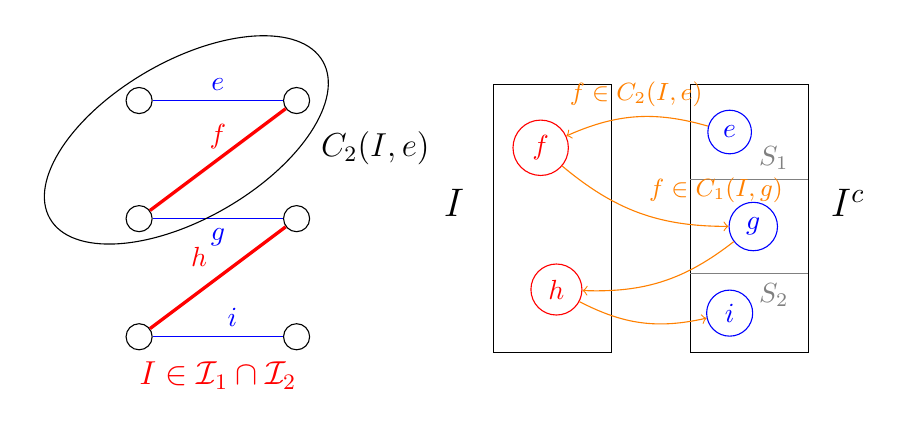
\begin{tikzpicture}
            \begin{scope}[
                    every node/.style={circle, draw},
                    % every edge/.style={draw, semithick}
                ]

                \node (l1) at (0,0) {};
                \node (l2) at (0,1.5) {};
                \node (l3) at (0,3) {};
                \node (r1) at (2,0) {};
                \node (r2) at (2,1.5) {};
                \node (r3) at (2,3) {};

                \node[red] (f) at (5.1,2.4) {$f$};
                \node[blue] (e) at (7.5,2.6) {$e$};
                \node[blue] (g) at (7.8,1.4) {$g$};
                \node[red] (h) at (5.3,0.6) {$h$};
                \node[blue] (i) at (7.5,0.3) {$i$};
            \end{scope}

            \draw[red, very thick] (l1) edge node[anchor=south east]{$h$} (r2);
            \draw[red, very thick] (l2) edge node[anchor=south]{$f$} (r3);
            \draw[blue] (l1) edge node[anchor=south west]{$i$} (r1);
            \draw[blue] (l2) edge node[anchor=north]{$g$} (r2);
            \draw[blue] (l3) edge node[anchor=south] {$e$} (r3);
            \draw[rotate around={30:(0.6,2.5)}] (0.6,2.5) ellipse (2 and 1);
            \node (ell) at (3,2.4) {\large$C_2(I,e)$};
            \node[red] (I) at (1,-0.5) {\large $I\in \mathcal I_1\cap \mathcal I_2$};

            \draw (4.5,-0.2) rectangle (6, 3.2);
            \draw (7,-0.2) rectangle (8.5, 3.2);
            \draw[gray] (7,2) edge node[anchor=south west]{$S_1$} (8.5, 2);
            \draw[gray] (7,0.8) edge node[anchor=north west]{$S_2$} (8.5, 0.8);
            \node (sqI) at (4,1.7) {\Large $I$};
            \node (sqIc) at (9, 1.7) {\Large $I^c$};
            \draw[->,orange] (e) edge [bend right=20] node[anchor=south] {\small$f \in C_2(I,e)$} (f);
            \draw[->,orange] (f) edge [bend right=20] node[anchor=south west] {\small$f \in C_1(I,g)$} (g);
            \draw[->,orange] (g) edge [bend left=20] (h);
            \draw[->,orange] (h) edge [bend right=20] (i);

        \end{tikzpicture}
        % \captionof{figure}{A graph with the spanning tree in black and arc subset $S$ in orange}
    \end{minipage}
\end{example}
\begin{assumption}
    From now on assume $S_1 \cap S_2 = \emptyset$.
    Otherwise, if there exists an $e \in S_1 \cap S_2$, then we could choose $I+e \in \mathcal I_1 \cap \mathcal I_2$ greedily.
\end{assumption}
\begin{observe}
    Given $I \in \mathcal I_1 \cap \mathcal I_2$.
    Using circuits, we can swap edges such that we stay at least in $\mathcal I_1$:
    Suppose $e \in S_1$ (and $e \not \in S_2$). Therefore, $C_2(I,e)-e \neq \emptyset$,
    meaning there is a $f \in C_2(I,e)-e$ which is also in $I$.
    In order to add $e$ to $I$, we must remove $f$.
    Consider $I - f$. We add $g \in I^c$ such that $f \in C_1(I,g) - g$, because
    deleting $f$ will remove the only possible circuit that can appear when adding $g$,
    therefore keeping $(I-f)+g \in \mathcal I_1$.
\end{observe}

We want to use previous observation along an augmenting path from $S_1$ to $S_2$
in order to generate an $I^\prime$ that is also in $\mathcal I_2$.
\begin{theorem} \label{thm:augm_path}
    We prove two parts:
    \begin{enumerate}
        \item As long as there is an augmenting path from $S_1$ to $S_2$ (i.e. a path of edges in a bipartite matching),
              we can augment our solution. \label{enum:augm_path}
        \item If there is no augmenting path, we are optimal. \label{enum:opt_path}
    \end{enumerate}
\end{theorem}
In order to prove the first part, we need a little bit more work first.
\begin{definition}
    Given a bipartite graph $(\{e_0,\dots,e_k\} \cup \{f_1,\dots,f_l\}, E)$.
    A path
    \[
        P = e_{i_0} \rightarrow f_{i_1} \rightarrow e_{i_1} \rightarrow \dots \rightarrow f_{i_s} \rightarrow e_{i_s}
    \]
    is \vocab{shortcut-free} if for every $i_j$ there is no larger index $i'>i_j$ such that $(e_{i_j},f_{i'}) \in E$
    or  $(f_{i_j},e_{i'}) \in E$.
\end{definition}
\begin{lemma}\label{thm:circuit-helper}
    Given a shortcut-free path, for all $i$ holds
    \begin{align*}
        C_1(I + e_0, e_i)\subseteq I \setminus \{f_1, \dots f_{i-1}\}+e_0+e_i
    \end{align*}
\end{lemma}
\begin{proof}
    Suppose the opposite. Then for some $i$ there exists a $j$ with $1 \leq j < i$ such that
    $f_j \in C_1(I,e_i)$, therefore $(f_j, e_i) \in E$. But $f_j \rightarrow e_i$ is a shortcut.
\end{proof}
\begin{definition}
    We define
    \begin{align*}
        I_i \coloneqq I \cup \{e_0, \dots, e_i\} \setminus \{f_1, \dots, f_i\}
    \end{align*}
    as the \vocab{partial augmentation}.
\end{definition}
\begin{lemma} \label{thm:part_augm}
    Given a shortcut-free full augmentation. For all $i$ holds $I_i \in \mathcal I_1$.
\end{lemma}
\begin{proof}
    We use induction over $i$. For $i=0$ this follows by $e_0 \in S_1$.
    Assume now $I_{i-1} \in \mathcal I_1$ and consider two cases:
    \begin{itemize}
        \item $I_{i-1}+e_i \in \mathcal I_1$:
              Then $I_i = I_{i-1}+e_i-f_i \in \mathcal I_1$ by subset stability.
        \item $I_{i-1}+e_i \not \in \mathcal I_1$: Then $C_1(I_{i-1},e_i) \neq \emptyset$.
              Observe by \autoref{thm:circuit-helper} that
              \[
                  C_1(I + e_0, e_i)\subseteq I \setminus \{f_1, \dots, f_{i-1}\}+e_0+e_i \subseteq I_{i-1}+e_i.
              \]
              By uniqueness of circuits, $C_1(I+e_0,e_i)=C_1(I_{i-1},e_i)$.
              As a result, $f_i \rightarrow e_i \in E$ iff $f_i \in C_1(I_{i-1},e_i)$,
              concluding $C_1(I_{i-1},e_i)-f_i \in \mathcal I_1$, and finally $I_i \in \mathcal I_1$.
    \end{itemize}
\end{proof}
\begin{corollary}
    If we augment on a shortcut-free path $P$, then $I^\prime \in \mathcal I_1 \cap \mathcal I_2$.
\end{corollary}
\begin{proof}
    For $I^\prime \in \mathcal I_1$ this follows directly from \autoref{thm:part_augm}.
    For $I^\prime \in \mathcal I_2$ we can derive an analoguous proof.
\end{proof}
This concludes part 1 of \autoref{thm:augm_path}.

For the second part, we want to prove optimality after termination of part 1.
Note that for $I \in \mathcal 1 \cap \mathcal 2$, the matroid rank function $r_i$ and any $S \subseteq E$
\begin{align*}
    |I^*| = |I^* \cap S| + |I^* \cap S^c| \leq r_1(S) + r_2(S^c),
\end{align*}
thus, tightness induces optimality of $I$. We want to find such $S$ for an maximal $I$:
\begin{lemma}
    Suppose $I^* \in \mathcal I_1 \cap \mathcal I_2$ does not have any augmenting path.
    Let $S$ be the set of nodes reachable via partial augmentation.
    Then
    \begin{enumerate}
        \item $|I^* \cap S^c| = r_2(S^c)$, and
        \item $|I^* \cap S| = r_1(S)$.
    \end{enumerate}
\end{lemma}
\begin{proof}
    Observe $S_1 \subseteq S^c$ and $S_2 \subseteq S$ by assumption of $I^*$.
    We prove both parts by contradiction.
    \begin{enumerate}
        \item Suppose strict inequality. By extensibility, we can add $e \in S^c \setminus I^*$
              to $I^* \cap S^c$ such that $(I^* \cap S^c) + e \in \mathcal I_2$.

              Notice $e \not \in S_2$, therefore $C_2(I^*, e) \neq \emptyset$ by definition, meaning there
              is $f \in C_2(I^*,e) - e \subseteq I^*$, but $f \not \in I^* \cap S^c$.
              Otherwise, $C_2(I^*,e) \subseteq  (I^* \cap S^c) + e$, and by subset stability $C_2(I^*,e) \in \mathcal I_2$, contradicting the circuit definition.

              As a consequence, $f \in I^* \cap S$, meaning $f$ is not reachable by definition of $S$,
              but a path $e \rightarrow f$ exists by definition of our matroid intersection graph - contradiction!
        \item Suppose strict inequality. By extensibility, we can add $e \in S \setminus I^*$
              to $I^* \cap S^c$ such that $(I^* \cap S) + e \in \mathcal I_1$.
              Analoguous, we can derive there is an $f \in I^* \cap S^c$ with a path $f\rightarrow e$,
              meaning $f$ is reachable, but $e$ is not by definition - contradiction!
    \end{enumerate}
\end{proof}
\begin{corollary}
    If $I^* \in \mathcal I_1 \cap \mathcal I_2$ does not have an augmenting path, then it is optimal.
\end{corollary}
\begin{remark}
    We can extend the cardinality case to arbitrary weighted intersection matroids.
    As a general idea, we can extend on the augmenting paths idea and additionally use successive shortest paths
    or the Hungarian Algorithm for a weighted bipartite matching.
    See \cite[Ch.~8]{comb-optimization-cook} for details.
\end{remark}
\begin{remark}
    We can use the same ideas for polymatroid and submodular intersection.
\end{remark}
Unfortunately, matroid-intersection cannot be efficiently extended to arbitrary numbers of matroids.
Intuitively, this can be explained because we cannot construct a basis with
Continuous One Property by glueing the parts together
as in the case with 2 matroids. This prohibits us from using Totally Dual Integrality.
\begin{theorem}
    Triple-matroid intersection is in $\NPC$, therefore cannot be solved efficiently.
\end{theorem}
\begin{proof}
    We can reduce from $\mathsf{HAMPATH}$. See the tutorial for the proof.
\end{proof}
As a closing thought, we want to have a last look at Totally Dual Integrality:
\begin{theorem}
    If $Ax \leq b$ is rational, then there is $q \in \integers$ such that $q^{-1}Ax \leq q^{-1}b$
    is Totally Dual Integral.
\end{theorem}
Nonetheless, this fact is useless since $q^{-1}b$ would have to be integral to get integer optimal solutions.
\begin{theorem}
    Given a rational polyhedron. Iff it can be written as a Totally Dual Integral system
    where $b$ is integral, then the polyhedron is integral.
\end{theorem}
\begin{proof}[Proof idea]
    We can add redundant constraints to "help" the dual.
\end{proof}
\begin{conclusion}
    Totally Dual Integrality is a property of the linear system, not the polyhedron.
\end{conclusion}